\documentclass{article}
\usepackage{graphicx}
\usepackage{hyperref}

\begin{document}
\section{introduction}
GFS is a scalable distributed file system for large distributed data-intensive
applications. It provides fault tolerance while running on inexpensive
commodity hardware, and it delivers high aggregate performance to a large
number of clients. Large deployments of GFS are capable of providing hundreds
of terabytes of storage across thousands of disks on over a thousand machines,
and it is concurrently accessed by hundreds of clients.

First, component failures are the norm rather than the
exception. The file system consists of hundreds or even
thousands of storage machines built from inexpensive commodity parts and is accessed by a comparable number of
client machines. The quantity and quality of the components virtually guarantee that some are not functional at
any given time and some will not recover from their current failures. We have seen problems caused by application
bugs, operating system bugs, human errors, and the failures
of disks, memory, connectors, networking, and power supplies. Therefore, constant monitoring, error detection, fault
tolerance, and automatic recovery must be integral to the
system.

Second, files are huge by traditional standards. Multi-GB
files are common. Each file typically contains many application objects such as web documents. When we are regularly
working with fast growing data sets of many TBs comprising
billions of objects, it is unwieldy to manage billions of approximately KB-sized files even when the file system could
support it. As a result, design assumptions and parameters
such as I/O operation and blocksizes have to be revisited

Third, most files are mutated by appending new data rather than overwriting
existing data. Random writes within a file are practically non-existent. Once
written, the files are only read, and often only sequentially. A variety of
data share these characteristics. Some may constitute large repositories that
data analysis programs scan through. Some may be data streams continuously
generated by running applications. Some may be archival data. Some may be
intermediate results produced on one machine and processed on another, whether
simultaneously or later in time. Given this access pattern on huge files,
appending becomes the focus of performance optimization and atomicity
guarantees, while caching data blocks in the client loses its appeal.

Fourth, co-designing the applications and the file system API benefits the
overall system by increasing our flexibility.  For example, we have relaxed
GFS’s consistency model to vastly simplify the file system without imposing an
onerous burden on the applications. We have also introduced an atomic append
operation so that multiple clients can append concurrently to a file without
extra synchronization between them. These will be discussed in more details
later in the paper.

 \section{Interface}
 GFS provides a familiar file system interface, but not POSIX semantics.
 Files are organized hierarchically in directories
 and identified by pathnames. The operations \texttt{create},
 \texttt{delete}, \texttt{open}, \texttt{close}, \texttt{read}, \texttt{write},
 and most interestingly, \texttt{append} to files is provided.

\section{Network architecture}

\begin{figure}
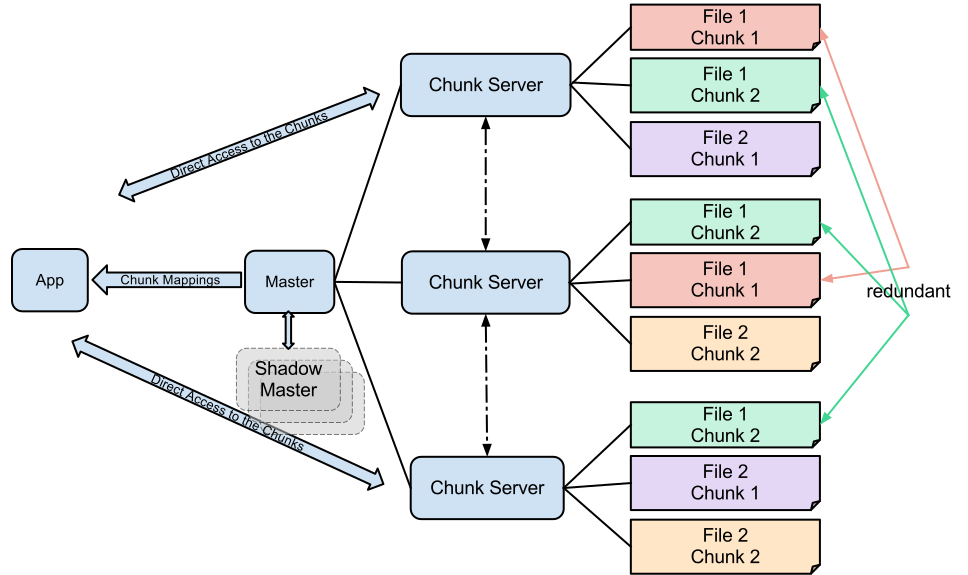
\includegraphics[width=\textwidth]{gfs-diagram.pdf}
\caption{GFS architecture}
\label{fig:architecture}
\end{figure}

On the server-side, there is a single \emph{master} controlling multiple slaves,
known as \emph{chunkservers}. These are accessed by multiple clients, as
shown in  Figure \ref{fig:architecture}.

\bibliographystyle{plain}
\bibliography{references}
\nocite{*}
\end{document}
